\documentclass[a4paper, 12pt]{article}%тип документа

%отступы
\usepackage[left=2cm,right=2cm,top=2cm,bottom=3cm,bindingoffset=0cm]{geometry}

%Русский язык
\usepackage[T2A]{fontenc} %кодировка
\usepackage[utf8]{inputenc} %кодировка исходного кода
\usepackage[english,russian]{babel} %локализация и переносы

%Вставка картинок
\usepackage{wrapfig}
\usepackage{graphicx}
\graphicspath{{pictures/}}
\DeclareGraphicsExtensions{.pdf,.png,.jpg}

%Графики
\usepackage{multirow}
\usepackage{pgfplots}
\pgfplotsset{compat=1.9}

%Математика
\usepackage{amsmath, amsfonts, amssymb, amsthm, mathtools}

%Заголовок
\author{Сифат Мд Абдуллах Ал Хасиб \\
Физтех школа электроники, фотоники и молекулярной физики \\
Группа Б04-105}
\title{\textbf{Лаборатория Работа 2.2.6 \\ Определение энергии активации по температурной зависимоти вязкости жидкости}}
\begin{document}
\maketitle
\section{Введение}\textbf{Цель работы}: Измерение скорости падения шариков при разной температуре жидкости; Вычисление вязкости жидкости по закону Стокса и расчет энергии активации.\\
\textbf{В работе используются}: Стеклянный цилиндр с исследуемой жидкостью (глицерин), термостат, секундомер, горизонтальный компаратор, микроскоп, мелкие шарики.
\section{Теоретическая справка}
По своим свойствам жидкости сходны как с газами, так и с твердыми телами. Подобно газам, жидкости принимают форму сосуда, в котором они находятся. Подобно твердым телам, они обладают сравнительно большой плотностью, с трудом поддаются сжатию.Двойственный характер свойств жидкостей связан с особенностями движения их молекул. В газах молекулы движутся хаотично, в их расположении отсутствует порядок. В кристаллических твердых
телах частицы колеблются около определенных положений равновесия -- узлов кристаллической решетки. В жидкостях, как и в кристаллах, каждая молекула находится в потенциальной яме электрического поля, создаваемого окружающими молекулами. Глубина потенциальной ямы в жидкостях больше средней кинетической энергии колеблющейся молекулы, поэтому молекулы колеблются вокруг более или менее стабильных положений равновесия. Однако у жидкостей различие между этими двумя энергиями невелико, так что молекулы нередко выскакивают из своей потенциальной ямы и занимают место в другой. В отличие от твердых тел, жидкости обладают  рыхлой структурой. В них имеются свободные места  -- дырки, благодаря чему молекулы могут перемещаться, покидая свое место и занимая одну из соседних дырок. В жидкостях такие переходы существенно замедлены. Количество молекул, имеющих энергии больше W, в соответствии с формулой Больцмана экспоненциально зависит от W. Температурная зависимость вязкости жидкости выражается формулой :

$$ \eta \approx Ae^{\frac{W}{kT}}$$\label{eq:viscosity}

Из формулы (\ref{eq:viscosity}) следует, что при повышении температуры вязкость должна резко понижаться.

Для исследования температурной зависимости вязкости жидкости в данной работе используется метод Стокса, основанный на измерении скорости свободного падения шарика в жидкости. Суть его заключается в следующем.

На всякое тело, двигающееся в вязкой жидкости, действует сила сопротивления. В общем случае величина этой силы зависит от многих факторов: от вязкости жидкости, от формы тела, от характера обтекания и т. д. Стоксом было получено строгое решение задачи о ламинарном обтекании шарика безграничной жидкостью. В этом случае сила сопротивления F определяется формулой

$$ F = 6\pi \eta rv,$$\label{eq:Stock's_force}

где $\eta$ - вязкость жидкости, $v - $ скорость шарика, $r - $ радиус шарика.

Рассматривая свободное падение шарика в вязкой жидкости, получаем уравнение:

$$Vg\left(\rho - \rho_{\text{ж}}\right) - 6\pi \eta rv = V\rho \frac{dv}{dt}$$\label{eq:Newton_second_law_for_ball}

Решая данное уравнение относительно скорости, получаем:

$$v\left(t\right) = v_{\text{уст}} - \left[v_{\text{уст}} - v\left(0\right)\right]e^{\frac{-t}{\tau}}$$\label{eq:velocity_equation}

$$v_{\text{уст}} = \frac{2}{9}gr^{2}\frac{\rho - \rho_{\text{ж}}}{\eta}$$ 

$$\tau = \frac{2}{9}\frac{r^{2}\rho}{\eta}$$

\section{Экспериментальная установка}
\begin{figure}[h!]
	\begin{center}
		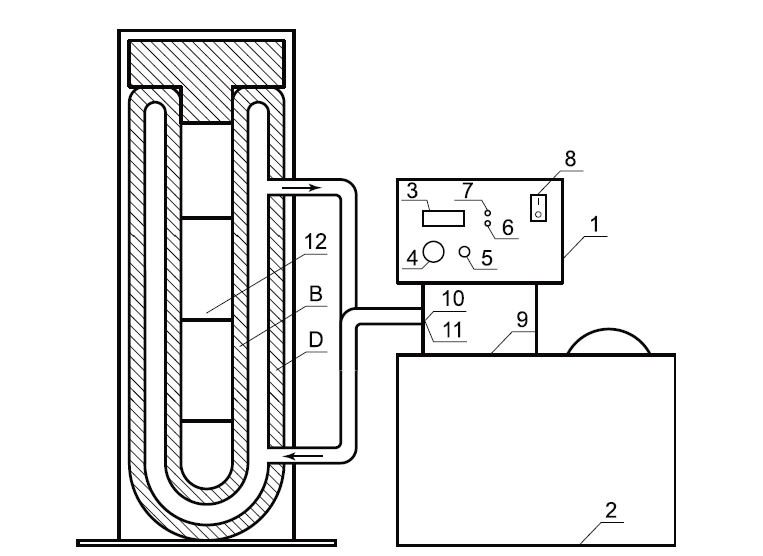
\includegraphics[width = 0.5\textwidth]{Fig.1.png}
		\caption{Схема экспериментальной установки}
		\label{fig:facility}
	\end{center}
\end{figure}
\newpage

\section{Экспериментальные данные}

Перед проведение эксперимента проведем измерения шариков, используемых в данном эксперименте.

Измерение диаметров шариков будем проводить с помощью микроскопа для двух групп шаров: стеклянных и металлических. Результаты занесем в таблицу (\ref{tab:results_of_diam_measuring})

\begin{table}[h]
\centering
\begin{tabular}{|c|c|c|}
\hline
№ измерения & \begin{tabular}[c]{@{}c@{}}Диаметр стеклянного\\ шарика, дел\end{tabular} & \begin{tabular}[c]{@{}c@{}}Диаметр металлического\\ шарика, mm\end{tabular} \\ \hline
1           & 2.20                                                                        & 0.80                                                                           \\ \hline
2           & 2.10                                                                        & 0.70                                                                 \\ \hline
3           & 2.0                                                                        & 0.90                                                                         \\ \hline
4           &  1.9                                                                       & 0.80                                                                           \\ \hline
5           & 2.0                                                                        & 0.70                                                                           \\ \hline
6           & 2.1                                                                        & 0.65                                                                           \\ \hline
7           & 2.0                                                                        & 0.80                                                                           \\ \hline
8           & 2.0                                                                        & 0.80                                                                           \\ \hline
9           & 2.08                                                                        & 0.70                                                                           \\ \hline
10          & 2.10                                                                        & 0.80                                                                           \\ \hline
11          & 2.06                                                                        & 0.76                                                                           \\ \hline
12          & 2.06                                                                        & 0.70                                                                           \\ \hline

\end{tabular}
\caption{Результаты измерения диаметров шариков}
\label{tab:results_of_diam_measuring}
\end{table}

Определим средние значения диаметров и погрешности их прямого измерения.

$$\overline{d_{\text{стекл}}}  = 2.1; \quad \overline{d_{\text{металл}}} = 0.70$$\label{eq:average_diam}

$$\sigma_{\text{стекл}} = 0.5;\quad  \sigma_{\text{металл}} = 0.3$$\label{eq:diam_mistake}

Как видно из (\ref{eq:diam_mistake}), случайная погрешность измерения диаметра шариков сильно больше систематической ошибки измерительного прибора, поэтому полная погрешность измерения диаметра $\approx$ случайной погрешности.

Затем проведем несколько серий измерений. Для каждой температуры проведем 8 измерений: по 4 для каждого типа шаров. результаты занесем в таблицы (\ref{tab:glass_balls_measuring}, \ref{tab:metal_balls_measuring}). Кроме того, в данные таблицы занесем также значение скоростей движения шаров, учитывая, что за измеренное время шары проходят расстояние $s = 9,9 $ см. Определим среднюю скорость, а также погрешность косвенного измерения средней скорости. Полученные данные будем использовать при расчете вязкости глицерина.
\newpage
\begin{table}[h]
\centering
\begin{tabular}{|c|c|c|c|c||c|c|c|c|c|}
\hline
$t_{1},$ c     & $t_{2},$ c   & $v,$ $\frac{\text{см}}{\text{с}}$   &$ \overline{v},$ $\frac{\text{см}}{\text{с}}$                & $\sigma_{\overline{v}}, $ $\frac{\text{см}}{\text{с}}$                &   $t_{1},$ c   & $t_{2},$ с    & $v,$ $\frac{\text{см}}{\text{с}}$    &$ \overline{v},$  $\frac{\text{см}}{\text{с}}$               & $\sigma_{\overline{v}}, $  $\frac{\text{см}}{\text{с}}$       \\ \hline
\multicolumn{5}{|c|}{ $t = 25,78^\circ C$}                                              & \multicolumn{5}{c|}{$t = 30,0^\circ C$}                                             \\ \hline
22.38 & 22.53 & 0,445 & \multirow{4}{*}{0,446} & \multirow{4}{*}{0,05} & 18.41 & 19.01 & 0.534 & \multirow{4}{*}{0,543} & \multirow{4}{*}{0,005} \\ \cline{1-3} \cline{6-8}
22.21 & 21.93 & 0,453 &                       &                       & 17.93 & 18.34 & 0.553 &                       &                       \\ \cline{1-3} \cline{6-8}
22.83 & 22.34 & 0,443 &                       &                       & 18.23 & 18.56 & 0.544 &                       &                       \\ \cline{1-3} \cline{6-8}
22.32 & 22.91 & 0,442 &                       &                       & 18.67 & 18.11 & 0.544 &                       &                       \\ \hline
\multicolumn{5}{|c|}{$t = 35,0^\circ C $}                                            & \multicolumn{5}{c|}{$t = 40,0^\circ C $}                                             \\ \hline
13.07 & 13.32 & 0,757 & \multirow{4}{*}{0,764} & \multirow{4}{*}{0,05} & 10.51 & 9.75 & 0,978 & \multirow{4}{*}{0,959} & \multirow{4}{*}{0,05} \\ \cline{1-3} \cline{6-8}
13.45 & 13.54 & 0,713 &                       &                       & 10.76 & 10.11 & 0,958 &                       &                       \\ \cline{1-3} \cline{6-8}
13.78 & 13.24 & 0,735 &                       &                       & 10,16 & 10,53 & 0,957 &                       &                       \\ \cline{1-3} \cline{6-8}
13.56 & 13.91 & 0,782 &                       &                       & 10,66 & 10,29 & 0,945 &                       &                       \\ \hline
\multicolumn{5}{|c|}{$t = 45,0^\circ C $}                                              & \multicolumn{5}{c|}{$t = 50,0^\circ C $}                                             \\ \hline
7,97  & 7,91  & 1,247 & \multirow{4}{*}{1,29} & \multirow{4}{*}{0,04} & 5.10 & 4.96 & 1.988 & \multirow{4}{*}{2.137} & \multirow{4}{*}{0,08} \\ \cline{1-3} \cline{6-8}
7,70  & 7,84  & 1,274 &                       &                       & 4.53 & 4.69 & 2.169 &                       &                       \\ \cline{1-3} \cline{6-8}
7,59  & 7,39  & 1,322 &                       &                       & 4.34 & 4.34 & 2.304 &                       &                       \\ \cline{1-3} \cline{6-8}
7,54  & 7,34  & 1,331 &                       &                       & 4.75 & 4.81 & 2.09 &                       &                       \\ \hline
\end{tabular}
\caption{Результаты измерения времени прохождения стеклянных шариков.}
\label{tab:glass_balls_measuring}
\end{table}

\begin{table}[h]
\centering
\begin{tabular}{|c|c|c|c|c||c|c|c|c|c|}
\hline
$t_{1},$ c     & $t_{2},$ c   & $v,$ $\frac{\text{см}}{\text{с}}$   &$ \overline{v},$ $\frac{\text{см}}{\text{с}}$                & $\sigma_{\overline{v}}, $ $\frac{\text{см}}{\text{с}}$                &   $t_{1},$ c   & $t_{2},$ с    & $v,$ $\frac{\text{см}}{\text{с}}$    &$ \overline{v},$  $\frac{\text{см}}{\text{с}}$               & $\sigma_{\overline{v}}, $  $\frac{\text{см}}{\text{с}}$       \\ \hline
\multicolumn{5}{|c|}{ $t = 25,78^\circ C$}                                              & \multicolumn{5}{c|}{$t = 30,0^\circ C$}                                             \\ \hline
30.38 & 30.87 & 0,326 & \multirow{4}{*}{0,347} & \multirow{4}{*}{0,05} & 18.41 & 19.01 & 0.534 & \multirow{4}{*}{0,543} & \multirow{4}{*}{0,005} \\ \cline{1-3} \cline{6-8}
30.43 & 30.23 & 0,347 &                       &                       & 17.93 & 18.34 & 0.553 &                       &                       \\ \cline{1-3} \cline{6-8}
30.45 & 30.21 & 0,354 &                       &                       & 18.23 & 18.56 & 0.544 &                       &                       \\ \cline{1-3} \cline{6-8}
30.32 & 30.45 & 0,342 &                       &                       & 18.67 & 18.11 & 0.544 &                       &                       \\ \hline
\multicolumn{5}{|c|}{$t = 35,0^\circ C $}                                            & \multicolumn{5}{c|}{$t = 40,0^\circ C $}                                             \\ \hline
13.07 & 13.32 & 0,757 & \multirow{4}{*}{0,764} & \multirow{4}{*}{0,05} & 10.51 & 9.75 & 0,978 & \multirow{4}{*}{0,959} & \multirow{4}{*}{0,05} \\ \cline{1-3} \cline{6-8}
13.45 & 13.54 & 0,713 &                       &                       & 10.76 & 10.11 & 0,958 &                       &                       \\ \cline{1-3} \cline{6-8}
13.78 & 13.24 & 0,735 &                       &                       & 10,16 & 10,53 & 0,957 &                       &                       \\ \cline{1-3} \cline{6-8}
13.56 & 13.91 & 0,782 &                       &                       & 10,66 & 10,29 & 0,945 &                       &                       \\ \hline
\multicolumn{5}{|c|}{$t = 45,0^\circ C $}                                              & \multicolumn{5}{c|}{$t = 50,0^\circ C $}                                             \\ \hline
7,97  & 7,91  & 1,247 & \multirow{4}{*}{1,29} & \multirow{4}{*}{0,04} & 5.10 & 4.96 & 1.988 & \multirow{4}{*}{2.137} & \multirow{4}{*}{0,08} \\ \cline{1-3} \cline{6-8}
7,70  & 7,84  & 1,274 &                       &                       & 4.53 & 4.69 & 2.169 &                       &                       \\ \cline{1-3} \cline{6-8}
7,59  & 7,39  & 1,322 &                       &                       & 4.34 & 4.34 & 2.304 &                       &                       \\ \cline{1-3} \cline{6-8}
7,54  & 7,34  & 1,331 &                       &                       & 4.75 & 4.81 & 2.09 &                       &                       \\ \hline
\end{tabular}
\caption{Результаты измерения времени прохождения металлических шариков.}
\label{tab:metal_balls_measuring}
\end{table}


\newpage
Определим значения вязкости глицерина в зависимости от температуры, а также тела, которое движется внутри глицерина. В теории, мы должны получить идентичные данные, так как вязкость не зависит от материала тела, движущегося в жидкости.

\begin{figure}[h!]
	\begin{center}
		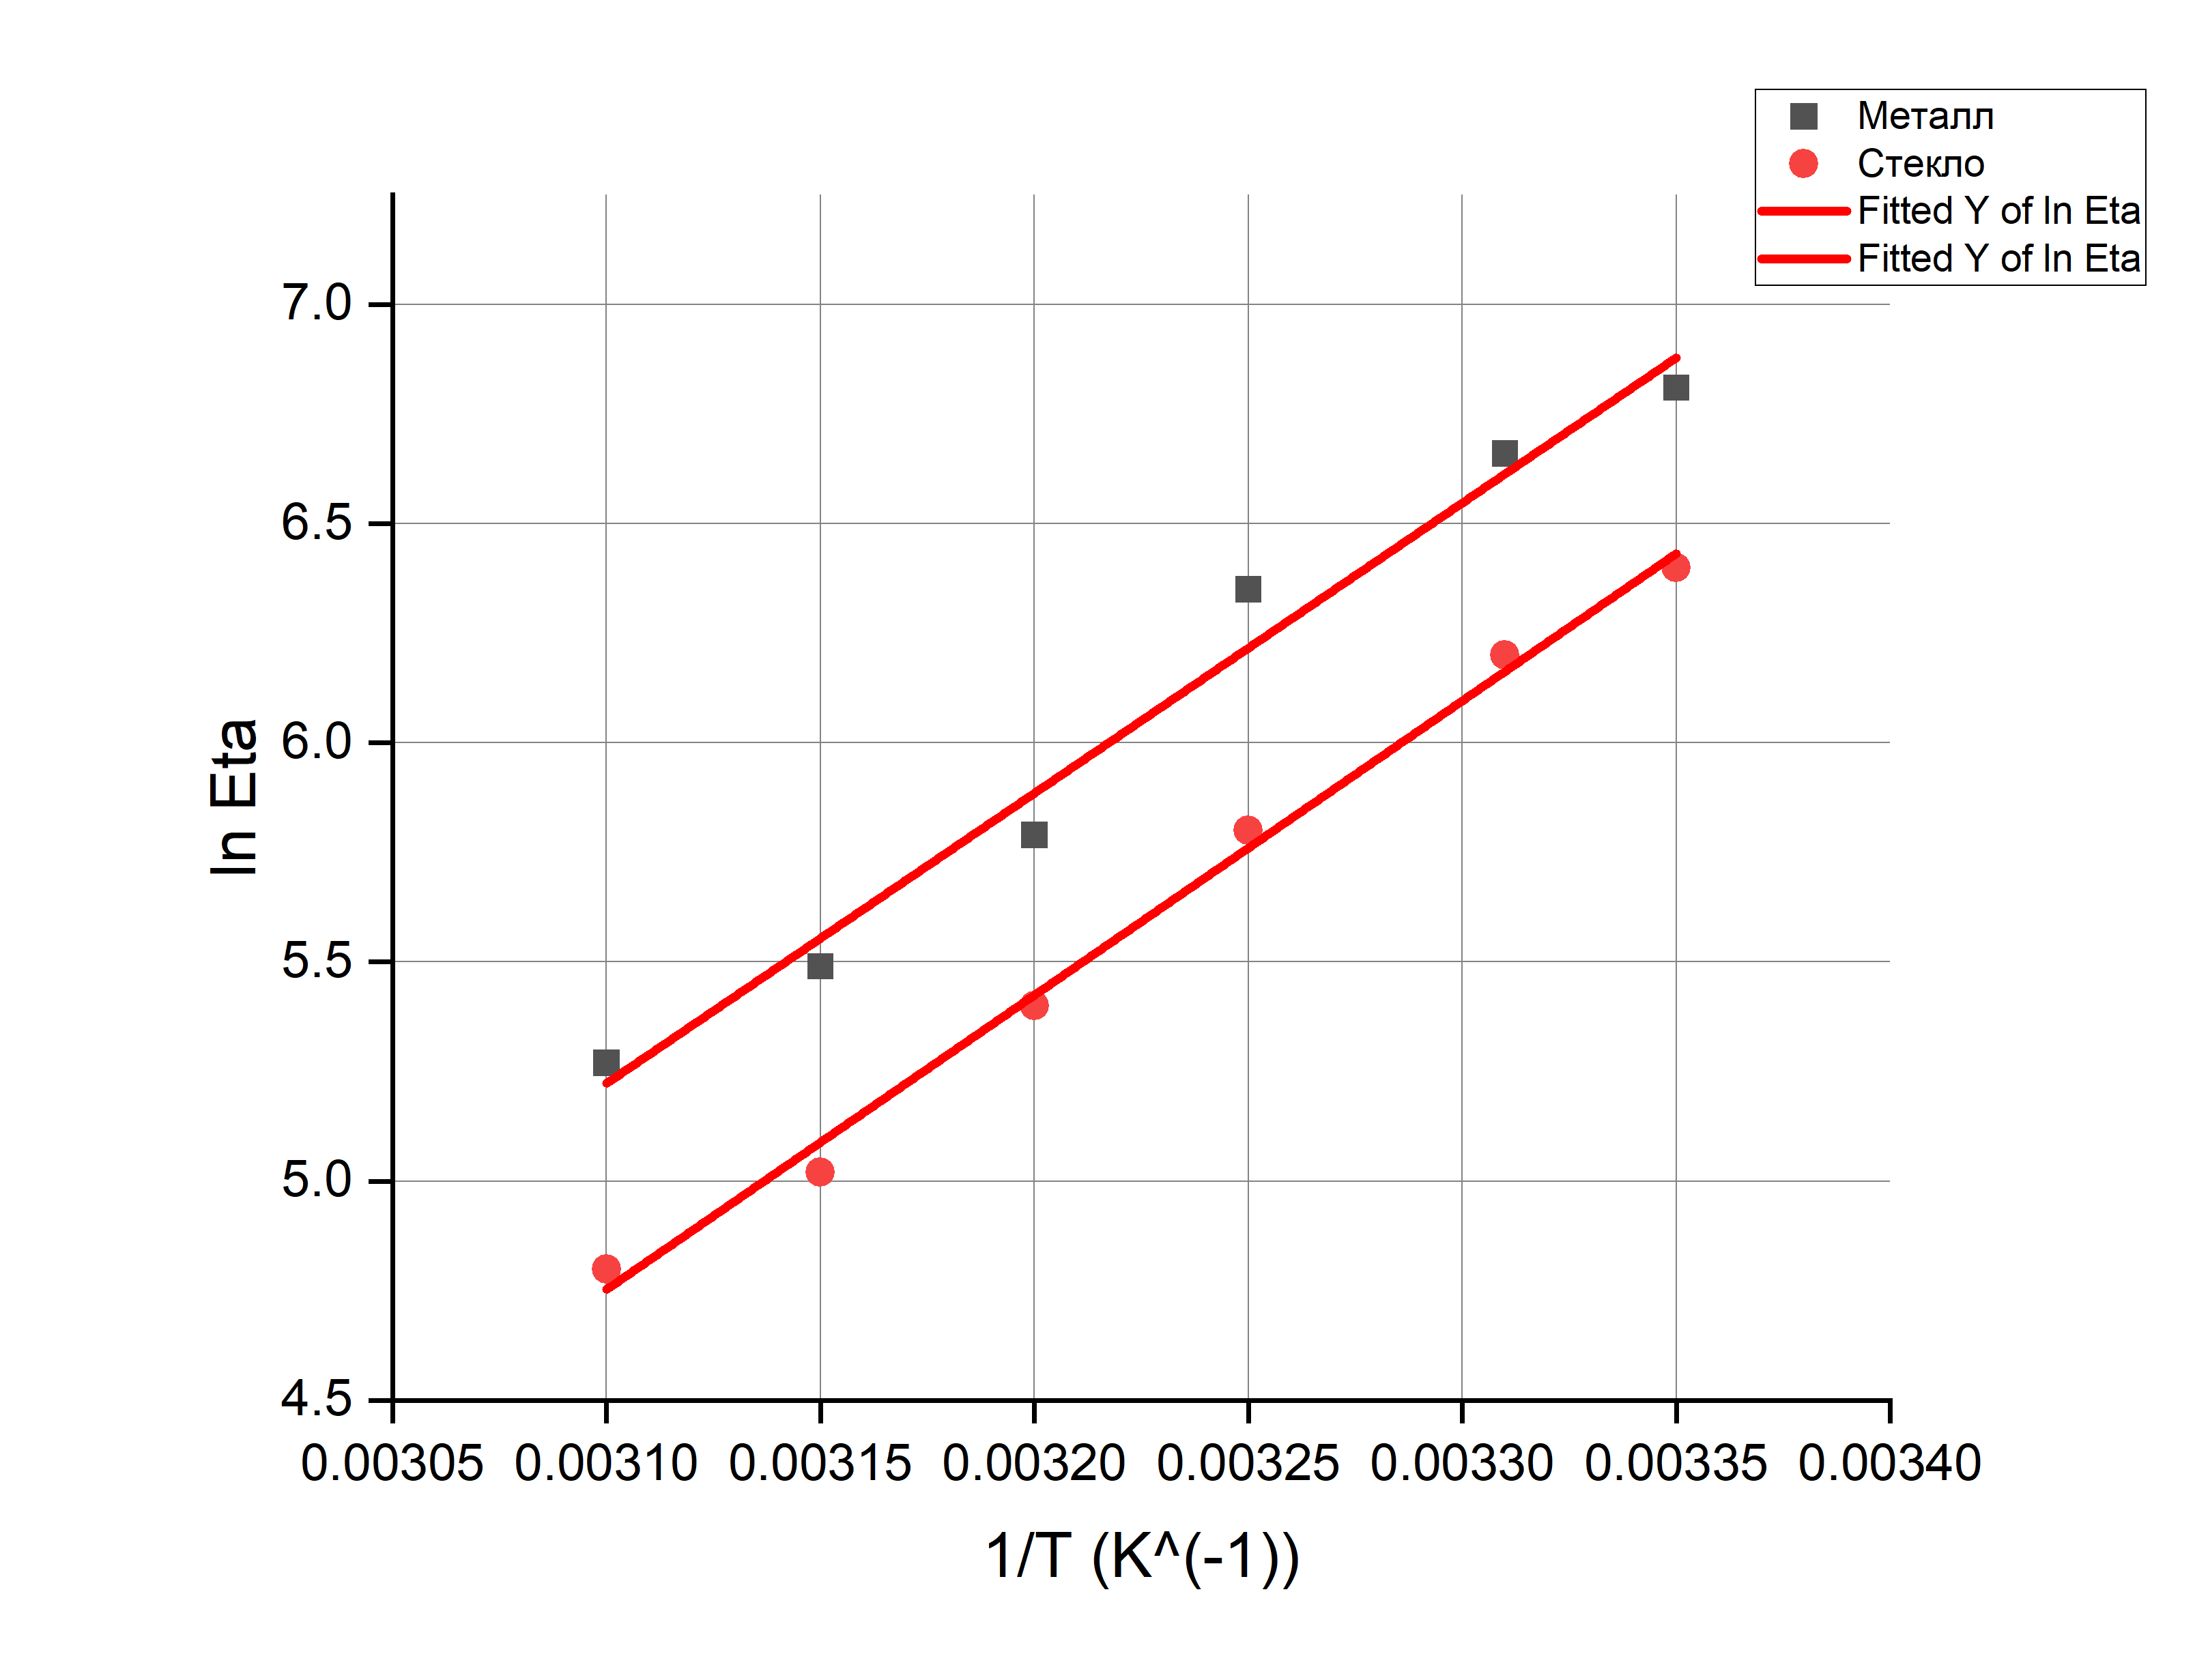
\includegraphics[width = 0.85\textwidth]{labphoto31.png}
		\caption{Графики зависимости логарифма вязкости от обратной температуры для двух серий измерений}
		\label{fig:graph_one}
	\end{center}
\end{figure}

Как видно из графиков, результаты, полученные с помощью металлических и стеклянных шаров дают одинаковые значения энергии активации, так как линейные приближения имеют одинаковый угол наклона, но стеклянные шарики позволяют вычислить вязкость воздуха точнее металлических. Для дальнейших расчетов будем использовать результаты, полученные на стеклянных шариках.

Используя значения углового коэффициента прямых, полученные с помощью МНК, определим значения энергии активации:

$$W = kT \cdot \alpha $$, $$W = 7,95\cdot 10^{-20}$$. 

Пользуясь МНК, также определяем погрешность определенной величины:

$$\sigma_{W} = 2,12 \cdot 10^{-21}$$

В итоге, полученное значение: $W = \left(8,0 \pm 0,2\right)\cdot 10^{-20} \frac{\text{Дж}}{\text{моль}}$;

Перейдем к определению числа Рейнольдса -- $Re$, для каждой серии опытов. Для этого вычислим вязкость глицерина при различных температурах. Данные (вместе со справочными) занесем в таблицу (\ref{tab:results}).

\begin{table}[h]
\centering
\begin{tabular}{|c|c|c|c|c|c|c|c|c|}
\hline
Температура  $^\circ C$     & 20   & 27,5 & 35  & 40  & 45  & 50  & 55  & 60  \\ \hline
$\eta, \text{Па} \cdot \text{с}$ & 1207 & 830  & 572 & 330 & 244 & 195 & 144 & 127 \\ \hline
\end{tabular}
\caption{Значения вязкости глицерина для различных температур.}
\label{tab:results}
\end{table}  

Результаты определения чисел Рейнольдса занесем в таблицу (\ref{tab:reynolds_number}).

\begin{table}[h!]
\centering
\begin{tabular}{|c|c|c|}
\hline
№ серии & $Re_{\text{стекло}}$ & $Re_{\text{металл}}$ \\ \hline
1       & 0,01                 & 0,01                 \\ \hline
2       & 0,02                 & 0,02                 \\ \hline
3       & 0,05                 & 0,04                 \\ \hline
4       & 0,14                 & 0,13                 \\ \hline
5       & 0,26                 & 0,24                 \\ \hline
6       & 0,40                 & 0,41                 \\ \hline
7       & 0,73                 & 0,71                 \\ \hline
8       & 0,94                 & 0,81                 \\ \hline
\end{tabular}
\caption{Значения чисел Рейнольдса для различных серий измерений}
\label{tab:reynolds_number}
\end{table}

Кроме того, полезно также определить значения времени релаксации шариков при движении в глицерине. Данные занесем в таблицу (\ref{tab:relax_time})

\begin{table}[h!]
\centering
\begin{tabular}{|c|c|c|}
\hline
№ серии & $\tau_{\text{стекло}}$, c & $\tau_{\text{металл}}$, c \\ \hline
1       & 0,55                   & 0,78                  \\ \hline
2       & 0,79                   & 1,14                  \\ \hline
3       & 1,15                   & 1,65                  \\ \hline
4       & 2,00                   & 2,86                  \\ \hline
5       & 2,70                   & 3,86                  \\ \hline
6       & 3,39                   & 4,84                  \\ \hline
7       & 4,57                   & 6,54                  \\ \hline
8       & 5,19                   & 7,42                  \\ \hline
\end{tabular}
\caption{Значения времени релаксации для различных серий измерений}
\label{tab:relax_time}
\end{table}
\newpage
\section{Заключение}

\begin{enumerate}
	\item В ходе выполнения работы была подтверждена теория силы вязкого трения, определяемая по формуле Стокса.
	\item Получены значения вязкости исследуемого образца (Глицерина) в зависимости от температуры. Данные значения хорошо согласуются с известными данными. Погрешность определения вязкости глицерина не превышает 30$\%$ (Наибольшая относительная погрешность определения вязкости - при температуре 60 $^\circ C$, сразу по нескольким причинам:
	
	Во-первых, как видно из таблицы (\ref{tab:reynolds_number}), при данной температуре уже нельзя считать движение шариков ламинарным.
	
	Во-вторых, само значение вязкости уже на порядок меньше, чем, например, при температуре 20 $^\circ C$, при практически не отличающейся абсолютной погрешности.
	
	В-третьих, большую погрешность в определение вязкости внесли металлические шарики, так как большое количество металлических шариков представляли несферические тела, на поверхности которых имелись выступы и раковины (Данный факт приводил к прилипанию пузырей воздуха к поверхности шарика, что существенно влияло на скорость движения шарика). Кроме того, относительно большую погрешность дало измерение времени движения, так как скорость была довольно большой, при малом значении вязкости.
	
	Кроме того, самое большое значение абсолютной погрешности измерения вязкости в серии с температурой 35$^\circ C$, что объясняется ошибкой измерения.
	\item Полученные значения чисел Рейнольдса позволяют утверждать, что при достаточно большой вязкости жидкости и малых геометрических размерах тела движение можно считать ламинарным.
	\item Полученные значения времени релаксации позволяют утверждать, что измеренное время прохождения конечного участка пути достоверны, так как время движения тел до начала данного участка больше, чем время релаксации.
	\item Несмотря на довольно большую погрешность итогового значения вязкости, геометрические размеры сосуда не оказали значимого влияния на движение шариков.
	\item Наибольшие вклады в погрешности косвенных измерений внесли погрешности измерения времени движения шариков (случайные ошибки).
\end{enumerate}







\end{document}